\documentclass{sigchi}

% Use this command to override the default ACM copyright statement (e.g. for preprints). 
% Consult the conference website for the camera-ready copyright statement.


%% EXAMPLE BEGIN -- HOW TO OVERRIDE THE DEFAULT COPYRIGHT STRIP -- (July 22, 2013 - Paul Baumann)
% \toappear{Permission to make digital or hard copies of all or part of this work for personal or classroom use is 	granted without fee provided that copies are not made or distributed for profit or commercial advantage and that copies bear this notice and the full citation on the first page. Copyrights for components of this work owned by others than ACM must be honored. Abstracting with credit is permitted. To copy otherwise, or republish, to post on servers or to redistribute to lists, requires prior specific permission and/or a fee. Request permissions from permissions@acm.org. \\
% {\emph{CHI'14}}, April 26--May 1, 2014, Toronto, Canada. \\
% Copyright \copyright~2014 ACM ISBN/14/04...\$15.00. \\
% DOI string from ACM form confirmation}
%% EXAMPLE END -- HOW TO OVERRIDE THE DEFAULT COPYRIGHT STRIP -- (July 22, 2013 - Paul Baumann)


% Arabic page numbers for submission. 
% Remove this line to eliminate page numbers for the camera ready copy
% \pagenumbering{arabic}


% Load basic packages
\usepackage{balance}  % to better equalize the last page
\usepackage{graphics} % for EPS, load graphicx instead
\usepackage{times}    % comment if you want LaTeX's default font
\usepackage{url}      % llt: nicely formatted URLs
\usepackage{makecell}
\usepackage{changepage}
\usepackage{mathtools}

% llt: Define a global style for URLs, rather that the default one
\makeatletter
\def\url@leostyle{%
  \@ifundefined{selectfont}{\def\UrlFont{\sf}}{\def\UrlFont{\small\bf\ttfamily}}}
\makeatother
\urlstyle{leo}


% To make various LaTeX processors do the right thing with page size.
\def\pprw{8.5in}
\def\pprh{11in}
\special{papersize=\pprw,\pprh}
\setlength{\paperwidth}{\pprw}
\setlength{\paperheight}{\pprh}
\setlength{\pdfpagewidth}{\pprw}
\setlength{\pdfpageheight}{\pprh}

% Make sure hyperref comes last of your loaded packages, 
% to give it a fighting chance of not being over-written, 
% since its job is to redefine many LaTeX commands.
\usepackage[pdftex]{hyperref}
\hypersetup{
pdftitle={SIGCHI Conference Proceedings Format},
pdfauthor={LaTeX},
pdfkeywords={SIGCHI, proceedings, archival format},
bookmarksnumbered,
pdfstartview={FitH},
colorlinks,
citecolor=black,
filecolor=black,
linkcolor=black,
urlcolor=black,
breaklinks=true,
}

% create a shortcut to typeset table headings
\newcommand\tabhead[1]{\small\textbf{#1}}


% End of preamble. Here it comes the document.
\begin{document}

\title{User-Defined Gesture for Flying Object}

\maketitle

\begin{abstract}
Nowadays, ways of interaction between human and computer are more diversified; however, these smart products are mostly immobile. With the development in the field of robotics and automation, intelligent products are no longer stationary. Although the present study of interactions are appropriate for tablet or smartphone, they have not yet been fully discussed in the field of flying objects. We presents a user-defined UAV gesture control study in outside without wearable device to collect user behavior. In all, 176 gestures from 16 participants in user study 1 were logged, analyzed and pair with think-aloud data for 11 commands performed, and then we built a taxonomy of 3D gestures . Based on our research findings, we discover that users tend to control UAVs by one hand instead of both, that a negative correlation was found between gesture complexities and their agreement, blahablahab blahablahab blahablahab blahablahab blahablahab blahablahab blahablahab blahablahab blahablahab blahablahab blahablahab blahablahab blahablahab blahablahab blahablahab blahabl

Our results will help designers and developers create better gesture sets informed by user behavior.
% Nowadays, ways of interaction between human and computer are more diversified; however, these smart products are mostly immobile. With the development in the field of robotics and automation, intelligent products are no longer stationary. Although the present study of interactions are appropriate for tablet or Smartphone, they are not yet been fully discussed in the field of flying objects. In this paper, we design a flying prototype that combined aircraft and webcam for human computer interaction called “Hummieye.” This paper presents a complete user-defined gesture set that relies on eliciting gestures from users including control the flying object, take a picture or video…etc. Also, we use the think-aloud method to understand users’ mental models when they perform the gestures. 
% Our experimental results discover that the gestures of most users will be limited to the prior experience of using a tablet or Smartphone. Nevertheless, we found that users will use different number of hands or fingers to interact with flying object based on the different distance. Moreover, users provide “unexpected” gestures when they fine tuning the flying object or asking it to perform some instruction. Our results will provide designers create better ways of interaction for flying object.Our results will help designers create better gesture control sets informed by user behavior.
\end{abstract}

\keywords{
	AR.Drone; UAV; Gestures; User-defined gesture
}

\category{H.5.m.}{Information Interfaces and Presentation}
: User Interfaces - \emph{Interaction styles, evaluation/methodology, user-centered design.}

\begin{figure}[!h]
\centering
\includegraphics[width=1\columnwidth]{userTask2.png}
\caption{A user performing a gesture to move the Parrot AR.Drone forward.}
\label{fig:userTask2}
\end{figure}

\section{Introduction}

Unmanned aerial vehicles (UAVs), also known as drones, are aircrafts whose flight is controlled remotely by a pilot or controlled autonomously by computers. Up to date, most people do not possess drones, aircrafts, flying objects, and so forth. Thus, the manipulation over or the interaction with a flying object remains unfamiliar to most people. The goal of this research is to cull, classify, and analyze intuitive gestures created by participants and to conclude the most favorable gestures for each function set of a UAV. We believe that drone manipulation by user-defined gestures should be fun and greatly reduce the learning curve resulting in improvements of human-drone interaction. Moreover, the results of this work provide drone designers, developers, and engineers an insight into such novel human-drone gestural interactions.
% Unmanned aerial vehicles (UAVs), also known as drones, are aircrafts whose flight is controlled remotely by a pilot or controlled autonomously by computers. A drone is a representation of technological advance and is commonly known for military use to reduce casualties. However, up to date, most people do not possess drones, aircrafts, flying objects, and so forth. Thus, the manipulation over or the interaction with a flying object remains unfamiliar to most people. Such unfamiliarity also leads to a paucity of previous works on human-drone interaction. Although some possessing flying objects such as low-price, small-sized, radio-controlled helicopters may have experiences on maneuvering its flight over a controller or a smartphone, the flying objects are usually used for games and entertainments instead of useful productivity and utility such as photography. Moreover, there still exists a steep learning curve to become a skillful pilot of a UAV with a controller or a smartphone. The goal of this research is to cull, classify, and analyze intuitive gestures created by participants and to conclude the most favorable gestures for each corresponding function (e.g., pitch, roll, and yaw) of a UAV. We expect that drone manipulation by user-defined gestures should be fun and greatly reduce the learning curve resulting in improvements of human-drone interaction. Moreover, the result of this work provides drone designers, developers, and engineers an insight into such novel human-drone interactions with expected gestures.

% There are three main control axes on the drone, including a longitudinal axis (roll), vertical axis (yaw), and lateral axis (pitch), controlling the drone to move left and right, forward and backward, and rotate in clockwise and counterclockwise, respectively. In addition, the change in rotational speed of the propellers in turn pushes the drone to a new altitude. Due to such hardware design of a drone, we asked participants to come up with gestures for these translational and rotational basic controls.

% Photographs are one of the most crucial memorabilia to keep track and share moments of our daily lives. Fortunately, some cheap, small-sized UAVs such as Parrot AR Drone equipped with cameras have made flying objects involve in the field of photography. Moreover, drones without being subject to topographical limitations have the advantage to fly to any position unreachable by man. Thus, users are able to take photos in a way that they never could before. Nevertheless, in order for UAVs to play a role in photography, drones should be easy to use, and its control methods must be natural and intuitive. We have confidence that gestures or body movements are one of the best control methods for UAVs where improvements on human-drone interaction and flying experience can be made. As a result, this study focuses on user-defined gestures, taxonomy of gestures, and the Likert-scale of gestures.

\section{RELATED WORK}
Wobbrock et al. \cite{Wobbrock:2009:UGS:1518701.1518866} conducted a study of gesture taxonomy for surface computing. His work provides important insight into the design of gestures for tablets. However, the gestures and its taxonomy concluded in this work were subject to 2D touch-screen devices without any further discussion involving 3D in-air gestures.

Vafaei \cite{Vafaei:2013} offered more detailed dimensions of gesture taxonomy. He proposed two main groups of the dimensions: gesture mapping and physical characteristics. Although Wobbrock et al.'s and Vafaei's works put stress on touch screens where no in-air gestures were found, the idea of the classification of gestures was quite inspirational for our study.

Hansen et al. \cite{Hansen:2014:UGC:2578153.2578156} explored four different gaze control modes to control a drone. Gaze interaction provides accessibility for disabled people. Nonetheless, the results of the work indicated that the participants mostly favored the mouse over gaze in terms of ease-of-use and reliability. Therefore, future work of similar topics is expected.

Graether and Mueller \cite{Graether:2012:JFR:2212776.2212386} provided preliminary insights into the design of a flying robot as a jogging companion. The insights includes four themes: embodiment, control, personality, and communication. Graether and Mueller discovered that the communication between the jogger and the flying robot is best through hand gestures.

Pfeil et al. \cite{Pfeil:2013:EGM:2449396.2449429} explored five 3D gesture metaphors for interaction with UAVs. Metaphors of proxy manipulation and seated proxy have the highest rating since the gesture sets are more natural, intuitive. Based on the results of their work, participants using gestural control were capable of completing the trial in less time compared to that using smartphone control. Such result is significant and tremendous for the field of human-computer interaction. However, the gesture sets defined by the author instead of users may not be the most intuitive and natural. We believe that user-defined gestures for drones should do even more improvements on the user experience.

% Wobbrock et al.\cite{Wobbrock:2009:UGS:1518701.1518866}conducted a study of gesture taxonomy for surface computing. Wobbrock recruited 20 participants to perform gestures for several tasks. He collected 1080 gestures and manually classified each gesture along four dimensions: form, nature, binding, and flow. Each dimension contains multiple categories. His work provides important insight into the design of gestures for tablets. However, the gestures and its taxonomy concluded in this work were subject to 2D touch-screen devices without any further discussion involving 3D in-air gestures.

% Vafaei \cite{Vafaei:2013} offered more detailed dimensions of gesture taxonomy. He proposed two main groups of the dimensions: gesture mapping and physical characteristics. Gesture mapping, including nature, form, binding, temporal, and context dimensions, involves how users map gestures to tasks. The group of physical characteristics focuses on the physical attributes of a gesture itself categorized into six dimensions: dimensionality, complexity, body part, handedness, hand shape, and range of motion. Although Wobbrock et al.'s and Vafaei's works put stress on touch screens where no in-air gestures were found, the idea of the classification of gestures was quite inspirational for our study.

% Hansen et al.\cite{Hansen:2014:UGC:2578153.2578156} explored four different gaze control modes to control a drone. Gaze interaction provides accessibility for disabled people. Drones may enable those with low mobility to quickly visually inspect surroundings or quickly obtain objects nearby. Nonetheless, the results of the work indicated that the participants mostly favored the mouse over gaze in terms of ease-of-use and reliability. Therefore, future work of similar topic is expected.

% Graether and Mueller \cite{Graether:2012:JFR:2212776.2212386} provided preliminary insights into the design of a flying robot as a jogging companion. The insights includes four themes: embodiment, control, personality, and communication. Graether and Mueller discovered that the communication between the jogger and the flying robot is best through hand gestures.

% Pfeil et al. \cite{Pfeil:2013:EGM:2449396.2449429} explored five 3D gesture metaphors for interaction with UAVs, including first person, game controller, the throne, proxy manipulation, and seated proxy. Metaphors of proxy manipulation and seated proxy have the highest rating since the gesture sets are more natural, intuitive and are metaphors of grasping the drone in user's hand. Based on the results of this work, participants using gesture control were capable of completing the trial in less time compared to that using smartphone control. Such result is significant and tremendous for the field of human-computer interaction. However, the gesture sets defined by the author instead of users may not be the most intuitive, natural. We believe that user-defined gestures for drones should do even more improvements on the user experience.
% returned to you to fix.

\section{USER STUDY}

\subsection{Developing Gesture Set}

Our user study was mainly divided into two parts, namely, Study 1 and Study 2. For Study 1, 16 participants were recruited and asked to think aloud and perform in-air gestures for each basic control (e.g. moving forward, backward, left, right, and so forth). After the gestures being developed, we then classified the gesture mappings along several dimensions in reference to the related works. For Study 2, another 16 participants were told to pick their favorite gestures from each gesture sets developed by the participants from Study 1.


\subsection{Referents and Signs}

We presented effects of 11 basic controls and 1 imaginative control (i.e., the referents) to 16 participants. All 11 basic controls included forward, backward, left, and right translation, rotation, ascending, descending, takeoff, landing, hovering, and activation of taking photos and recording videos based on the the functionality of a drone. The imaginative control, pointing to specified destination, was the assignment for the Drone to fly to a specific spot in a 3D space. We asked all participants to invent all 13 corresponding gestures (i.e., the signs) in Study 1.

\subsection{Apparatus}

Parrot AR Drone 2.0, a quadrotor vehicle, equipped with a camera facing was chosen as the flying object since it is popular, programmable, and affordable. FreeFlight app is the official smartphone app allowing joystick-like control made by Parrot SA. There are also several third-party open source projects so that it comes in handy for further system implementation.

\subsection{Participants}

32 paid participants with age ranging from 19 to 25 volunteered for the study. None had experience with piloting a flying object. All were right-handed and were college students recruited from various fields. Half of the participants consisting of 6 females and 10 males attended Study 1 for gesture set development. The other half consisting of 6 females and 10 males took part in Study 2 for gesture voting. 

% \begin{figure}[!h]
% \centering
% 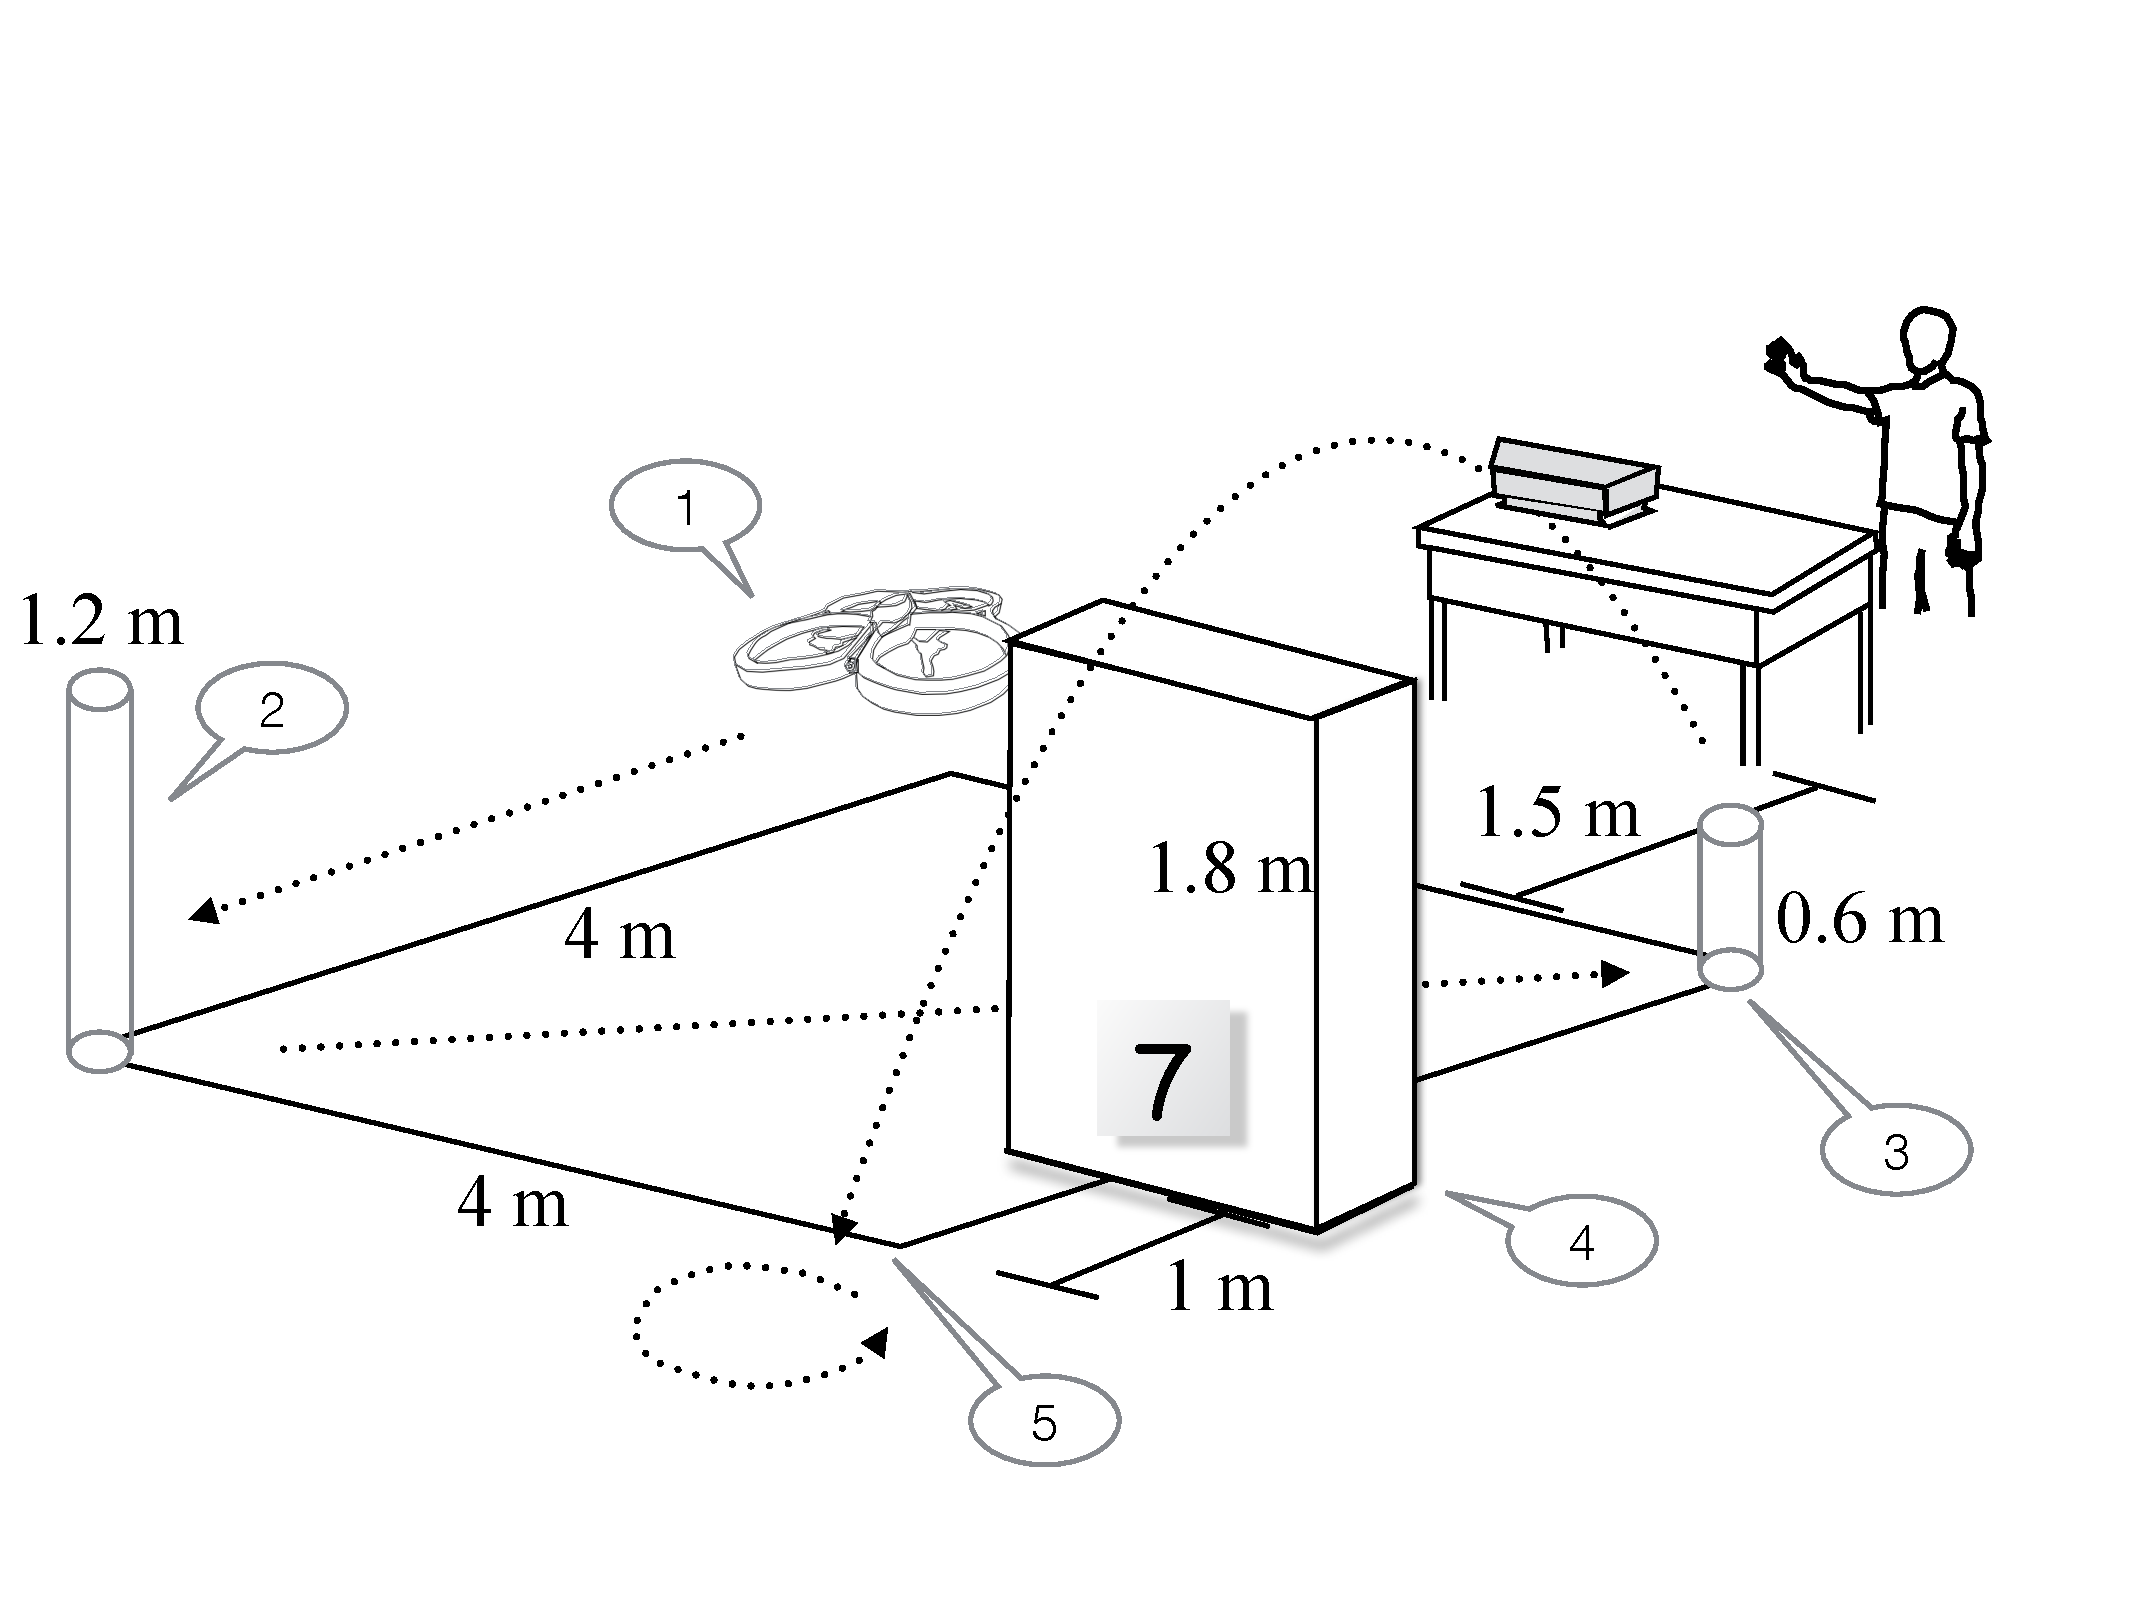
\includegraphics[width=1\columnwidth]{TaskFigure.pdf}
% \caption{Our test space was approximately 4 m long, and 4 m wide. The participant was placed away from the area for a full view of the test space. At location 1 was where the Drone began to take off. At location 2 and location 3 were two lightweight columns with 1.2 m and 0.6 m in height, both made of empty beverage cans stacking up. Location 4 was a 1.8 m-high obstacle made of stacked grocery boxes.}
% \label{fig:taskfigure}
% \end{figure}

% \subsection{Trial Design}

% The trial designed by Pfeil et al.\cite{Pfeil:2013:EGM:2449396.2449429} was to ask users to stand in front of a Kinect device, use gestures to fly the Drone to the 4 corners of a rectangular test space, and eventually land on a designated spot within the test space. We designed our trials for Study 2 in a similar manner (Figure\ref{fig:taskfigure}). First, after the Drone took off at location 1, the participant was asked to push and topple the columns with the Drone at location 2 and 3 in sequence. The toppling of the columns functioned as a confirmation of checkpoint that the Drone had reached the specified spot. Moreover, the columns with different height were designed for the participants to make use of the ascend-descend gesture control. Then, the Drone should fly over the obstacle at location 4. Behind the obstacle was a piece of paper written with a number that was not visible from the participant's viewpoint. Thus, the participant should fly to location 5, rotate the Drone, and read the number through the computer screen receiving live pictures from the camera of the Drone. After reading the number, the Drone landed immediately, and the trial was completed. If the Drone crashed during the trial, the Drone would take off at the crash site and continue the rest of trial. Each participant completed the trial 5 times.

% \begin{figure*}
%   \centering
%   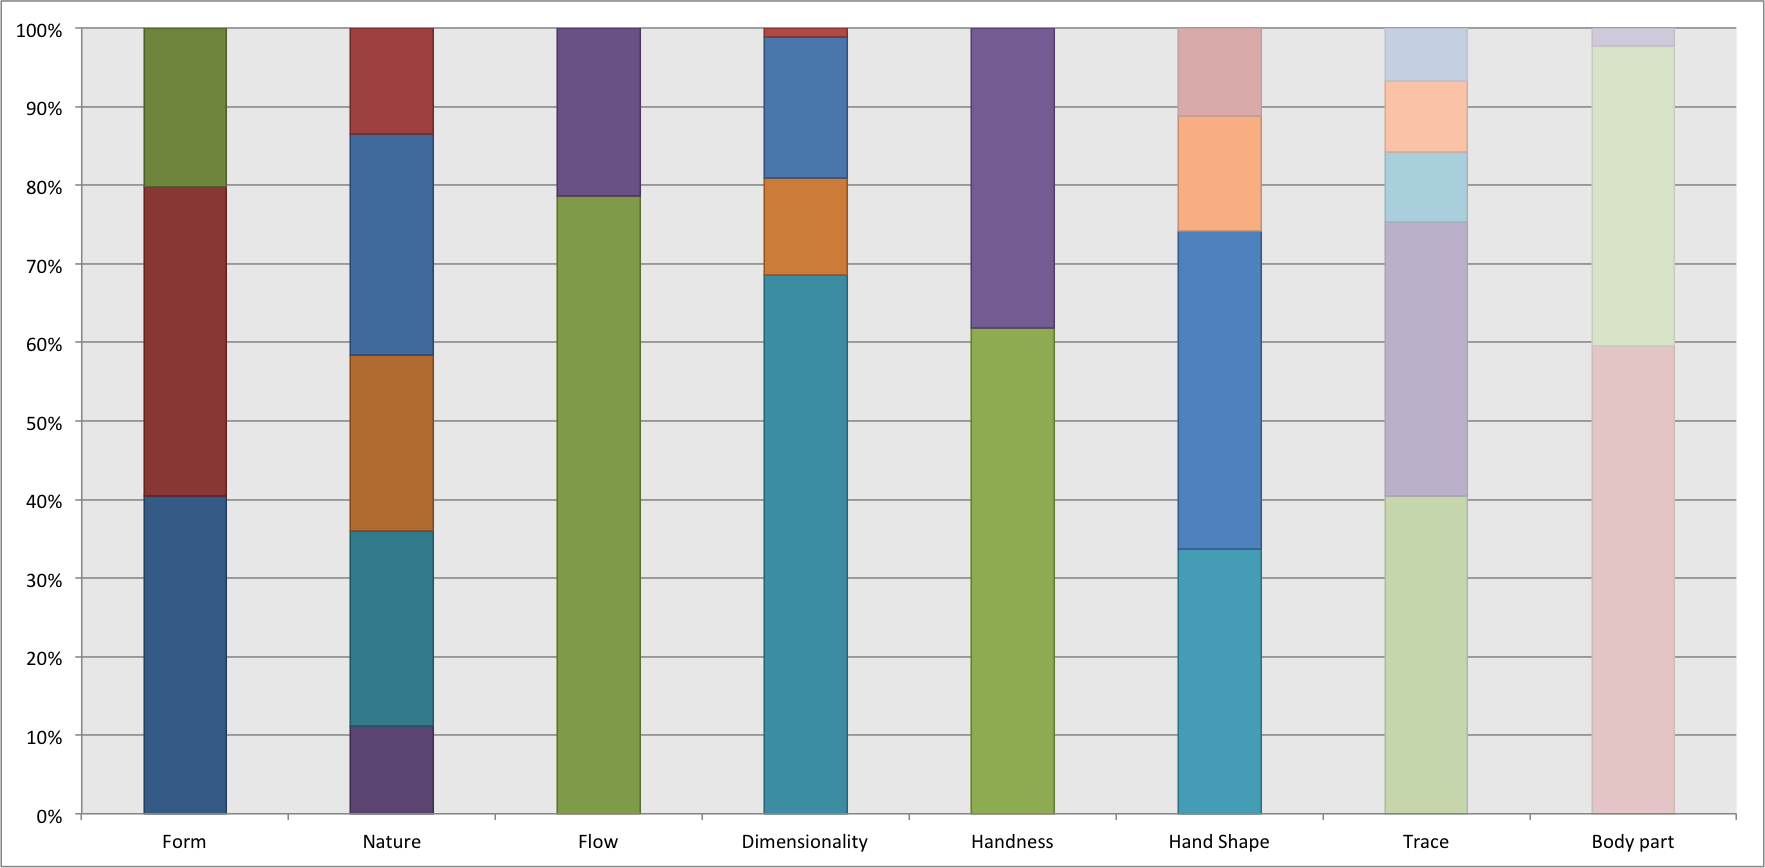
\includegraphics[width=1\textwidth]{taxonomy.png}
%   \caption{The user-defined game control set with \emph{In-Air} interaction, The percentage indicate the portion of users who perform the control action for the game task.}
%   \label{fig:InAirSet}
%   \end{figure*}


\subsection{Procedure}

In Study 1, an approximate 90-second short video of the introduction and motivation of this project was played in the beginning. Second, another 60-second short video showed how the drone moved. Then, the participant was asked to stand up and start to come up with 13 gestures for all 13 controls in random order. We allowed the participant to change any previously defined gesture if a new idea came to mind. After all gestures being developed, we employed a Wizard of Oz approach to give the participant an idea of how the interaction worked.

After Study 1, we categorized the user-defined gesture sets. Since the gesture for left and right were "symmetric", and so were that for ascend and descend, we grouped them into left-right and ascend-descend gesture sets, respectively, leading to 11 gesture sets. All the actions of all 11 gesture sets were recorded in a video which was played for all participants to pick their favorite gesture for each gesture set in Study 2.

\begin{table}
  \centering
  \begin{adjustwidth}{-0.4cm}{}
  \begin{tabular}{|l|l|l|}
    \hline
    \multicolumn{3}{|p{1.06\columnwidth}|}{\centering\tabhead{\textbf{Taxonomy of Gesture Set}}}\\
    \Xhline{4\arrayrulewidth}
    \em{Form} &Static& No motion occurs in G.\\ \cline{2-3}
    &Large-scale& substantial motion occurs in G. \\ \cline{2-3}
    &Small-scale& little motion occurs in G.\\
    \Xhline{4\arrayrulewidth}
    \em{Nature} & Symbolic &visually depicts a sign \\ \cline{2-3}
    &Pantomimic&Imitates real meaningful actions.\\ \cline{2-3}
    &Pointing&Points to a specific direction.\\ \cline{2-3}
    &Manipulative&Directly manipulates the object.\\ \cline{2-3}
    &Abstract&Mapping is arbitrary.\\
    \Xhline{4\arrayrulewidth}
    \em{Flow} & Discrete&Action is performed after G.\\ \cline{2-3}
    &Continuous&Action is performed during G.\\ 
    \Xhline{4\arrayrulewidth}
    % \em{Dimensionality} & Single-axis & G. occurs around a single axis.\\ \cline{2-3}
    % &Double-axis&G. occurs on a surface.\\ \cline{2-3}
    % &Tri-axis&G. involves either translational or\\&& rotational motion, not both.\\ \cline{2-3}
    % &Six-axis&G. occurs around both \\&&rotational and translational axes.\\
    % \Xhline{4\arrayrulewidth}
    \em{Handedness} & Dominant & G. is performed by the \\&&user's dominant hand/arm \\ \cline{2-3}
    &Bi-manual&G. is performed using \\&&both hands/arms\\
    \Xhline{4\arrayrulewidth}
    \em{Hand Shape} &&Free hand, ball holding, bent hand,\\&& Fist,pinch, Open hand
    index finger,\\&&Fhumb finger, Flat hand, ASL-F,\\&&ASL-C, ASL-L, ASL-O, \\&&ASL-V, ILY\\
    \Xhline{4\arrayrulewidth}
    \em{Trace}&Straight line&Moving parts trace a straight line.\\ \cline{2-3}
    &Fan shape&Moving parts trace a fan shape.\\ \cline{2-3}
    &Cone&Moving parts trace a cone.\\ \cline{2-3}
    &Expansion/&Hand posture changes with \\&Contraction&expansion or contraction.\\
     \cline{2-3}
    &Traceless&G. is static.\\
    \Xhline{4\arrayrulewidth}
  \end{tabular}
  \caption{"G." means "Gesture"}
  \label{tab:classificationTable}
  \end{adjustwidth}
\end{table}

\begin{figure}[!h]
\centering
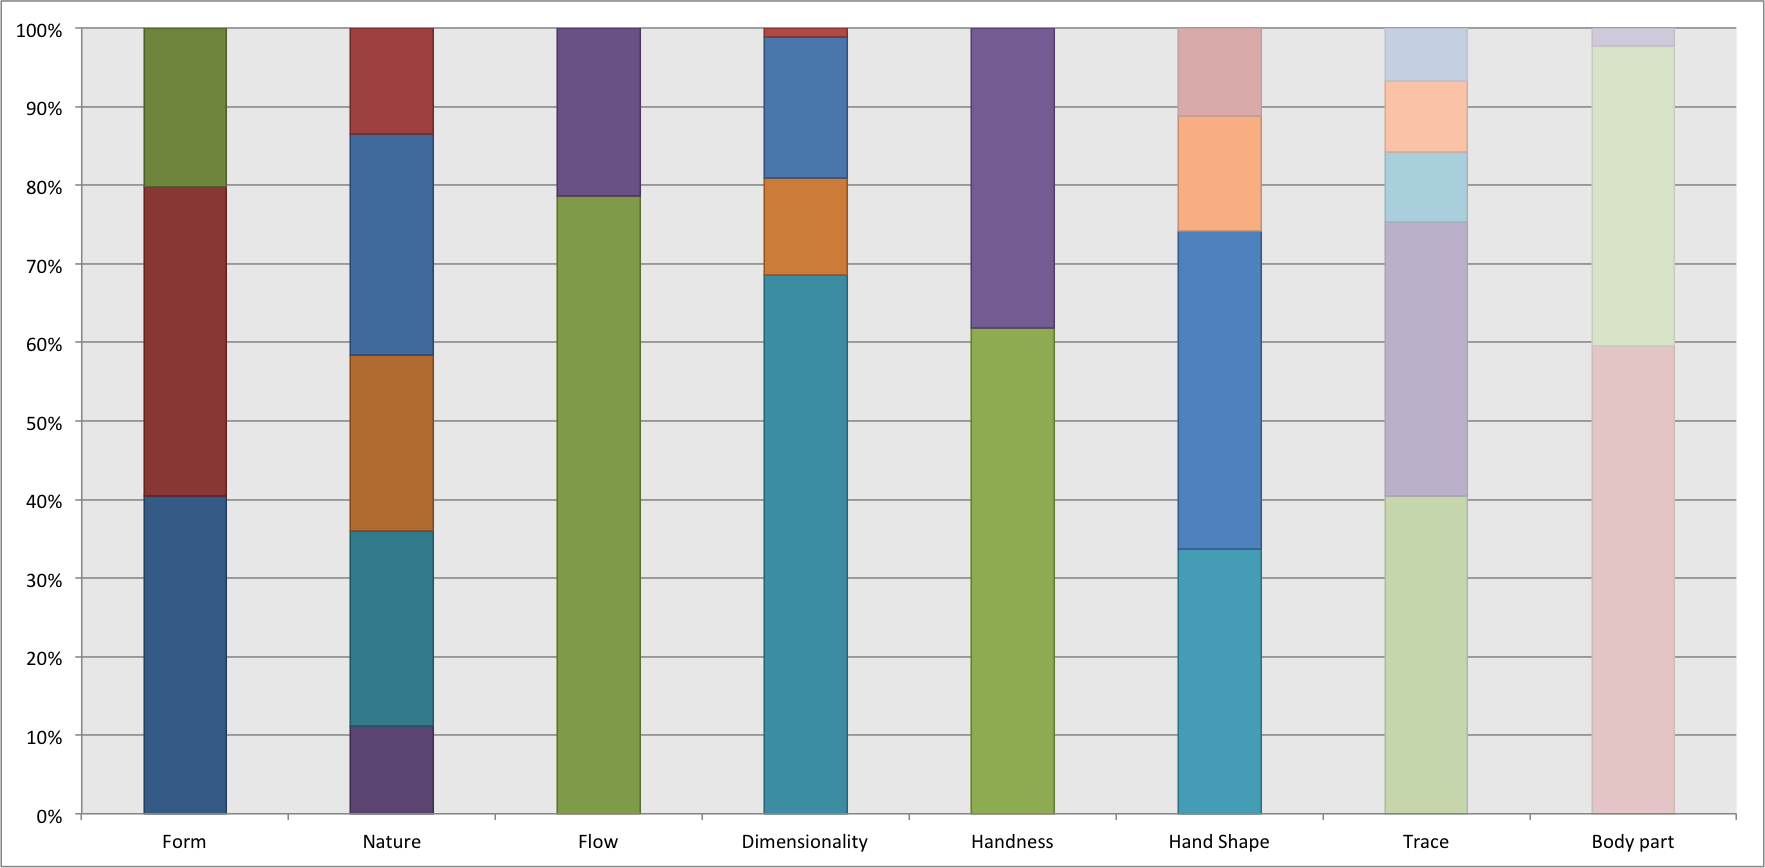
\includegraphics[width=1\columnwidth]{taxonomyFigure.png}
\caption{Percentage of gestures in each taxonomy category.}
\label{fig:taxonomyFigure}
\end{figure}

\section{RESULT \& DISCUSSION}

\subsection{Classification of 3D Gestures}
Gesture taxonomy has been used in several works involving speech gestures, sign language, touch screen gestures, and so forth. However, works involving gestures for flying object seemed rare lately. We managed to explore the most intuitive gestures for UAVs and provide future developers insights for better control methods.

In reference to related works, we manually classified each gesture along six dimensions: form, nature, flow, handedness, hand shape, and trace. All the gestures were performed by participants from Study 1. Each dimension contains multiple categories, shown in Table \ref{tab:classificationTable}.

The dimension of form describes the motions of all gestures. It is important to find out how many body parts are involved so that future developers will choose appropriate sensor devices to capture the motion.

The nature dimension conveys how UAVs are regarded and how a user interacts with them. A user would express with a symbolic gesture or a pantomimic gesture if a drone is regarded as more of a human. On the contrary, a user would perform a pointing gesture or a manipulative gesture if a drone is regarded as more of an object. Finally, abstract gestures are with arbitrary mappings for which no obvious concept human or object is considered.

In the flow dimension, a gesture would be continuous if the task is performed during gesticulation. In contrast, if a gesture is discrete, the gesture must be completed first and subsequently bring out the desired task. Thus, the input sampling rate and real-time gesture recognition are important factors to achieve a functional system.

The handedness dimension describes the involvement of the user's dominant hand and non-dominant hand for each task. In our study, no participant performed gestures specifically for the non-dominant hand, so future developers should focus on dominant-hand gestures.

The hand shape dimension describes the configuration, form, and posture of fingers as performing a gesture. We discovered that participants asked for specific hand shapes to perform specific tasks. Therefore, hand shape recognition should be considered and be part of future system implementation while it is mostly neglected in related works. The hand shapes listed in Table \ref{tab:classificationTable} were in reference of Vafaei's work \cite{Vafaei:2013}.

The trace dimension describes a variety of shapes traced by the moving parts of a gesture. The future drone system should analyze and recognize these traces after capturing the users' motion. The traces are shown in Figure \ref{fig:GestureSetFigure}.

% The handedness dimension describes the involvement of the user's dominant hand and non-dominant hand for each task. In our study, no participant performed gestures specifically for the non-dominant hand, so the non-dominant category is no needed. Participants performed gestures either with the dominant hand or both hands.

% The hand shape dimension describes the configuration, form, and posture of fingers as performing a gesture. Some hand shapes were performed including free hand, ball holding, bent hand, fist, pinch, open hand, index finger, thumb finger, flat hand, ASL-F, ASL-C, ASL-L, ASL-O, ASL-V, and ILY in reference of Vafaei's work \cite{Vafaei:2013}. For example, to have the drone moving away from the user is to perform a gesture with a flat hand. Another example would be performing a gesture with a ASL-V hand shape for activation of taking pictures.

% The trace dimension describes a variety of shapes traced by the moving parts of a gesture. Traces include straight line, fan shape, cone, hand shape expansion and contraction, and traceless. The traces are shown in FIGURE X.


  \begin{table}
    \centering
    \begin{adjustwidth}{}{}
    \begin{tabular}{|l|l|l|}
      \hline
      \tabhead{Referents} &
      \multicolumn{1}{|p{0.13\columnwidth}|}{\centering\tabhead{Mean}} &
      \multicolumn{1}{|p{0.13\columnwidth}|}{\centering\tabhead{Std.}} \\
      \hline
      Ascend and Descend & 1.00 & 0 \\
      \hline
      Forward & 1.25 & 0.50\\
      \hline
      Left and Right & 1.50 & 1.00 \\
      \hline
      Backward & 1.50 & 0.58 \\
      \hline
      Take pictures & 2.25 & 0.50 \\
      \hline
      Land & 2.75 & 0.96 \\
      \hline
      Take off & 3.00 & 0.82 \\
      \hline
      Record videos & 3.00 & 0.82 \\
      \hline
      Hover & 3.25 & 1.26 \\
      \hline
      Point to specified destination & 3.50 & 1.73 \\
      \hline
      Rotate & 3.50 & 0.58 \\
      \hline
      \bf{Mean} & \bf{2.41} & \bf{0.79}\\
      \hline
    \end{tabular}
    \caption{The 11 commands for which participants chose gestures. Each command’s conceptual complexity was rated by the 4 authors (1=simple, 5=complex). During the study, each command was presented with an animation and recorded verbal description.}
    \label{tab:complexityTable}
  \end{adjustwidth}
  \end{table}

\subsection{Agreement}

After all 16 participants had provided gestures for each referent for Study 1, we grouped the gestures within each referent such that each group held identical gestures. Group size was then used to compute an agreement score A that reflects, in a single number, the degree of consensus among participants.

\begin{equation}
A = \frac{\displaystyle{\sum_{r\epsilon R }} \sum_{P_i \subseteq P_r } \left(\frac{\lvert{P_i}\rvert}{\lvert{P_r}\rvert}\right) ^ 2}{\displaystyle{\lvert{R}\rvert}}
\end{equation}

In Eq. 1, r is a referent in the set of all referents R, Pr is the set of proposed gestures for referent r, and Pi is a subset of identical gestures from Pr. The range for A is $\left[\lvert{P_r}\rvert ^{-1}, 1\right]$. As an example, consider agreement for forward in study 1 and study 2. Both had five groups of identical gestures. The former had groups of size 1, 10, 2, 1, and 2.
\begin{equation}
   A_{forward} = 2\left(\frac{1}{16}\right) ^ 2  + \left(\frac{10}{16}\right) ^ 2 + 2\left(\frac{2}{16}\right) ^ 2 = 0.48
\end{equation}

% For study 2, we compute

% \begin{equation}
%    A_{forward2} = \left(\frac{11}{16}\right) ^ 2  + \left(\frac{3}{16}\right) ^ 2 + 2\left(\frac{1}{16}\right) ^ 2 = 0.52
% \end{equation}

\begin{figure}[!h]
\centering
\includegraphics[width=1\columnwidth]{Agreement-2.pdf}
\caption{Agreement for each referent sorted in descending order according to complexity rated by the 4 authors.}
\label{fig:agreementFigure}
\end{figure}

The result of agreement is indicated in Figure \ref{fig:agreementFigure}. The overall agreement for Study 1 gestures was $A=0.22$. Gesture complexities correlated inversely with their agreement, as more complex referents elicited lesser gestural agreement.

\subsubsection{Finding}
\begin{figure*}
  \centering
  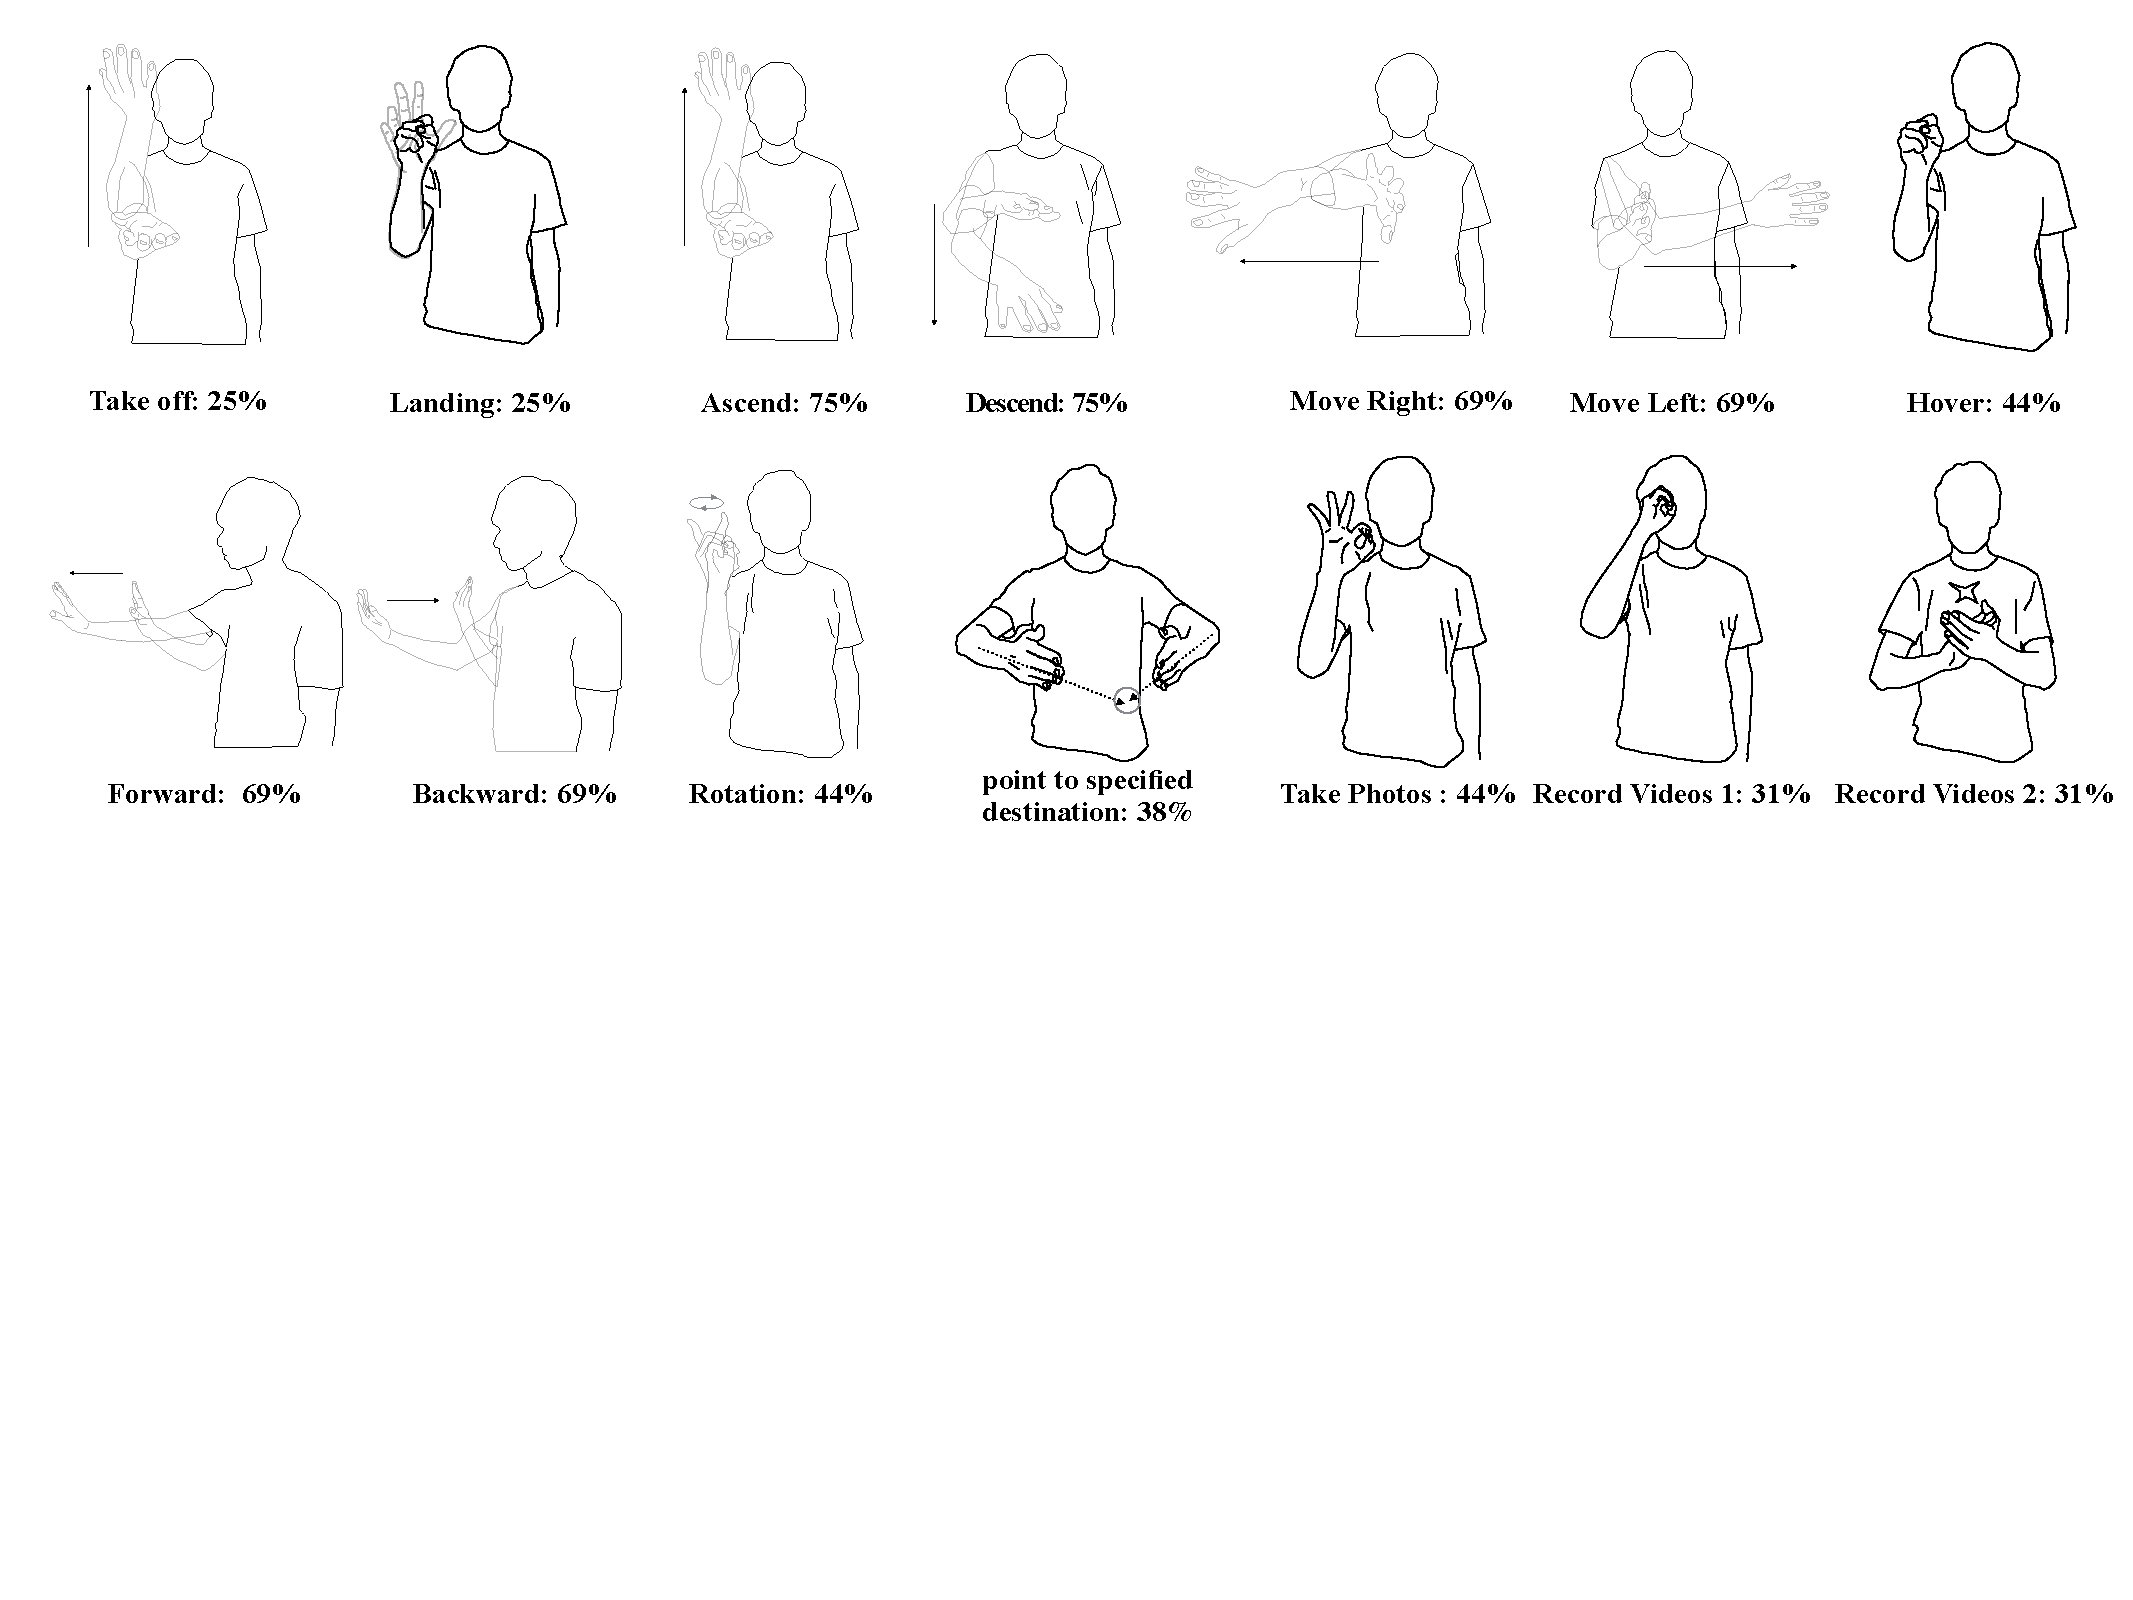
\includegraphics[width=1\textwidth]{GestureSetFigure1.pdf}
  \caption{Top gestures for each task in user study 2.}
  \label{fig:GestureSetFigure}
  \end{figure*}
The statistical result of Figure \ref{fig:agreementFigure} shows that most of the basic movement controls involving translation along the pitch, roll, or yaw axes such as forward and backward, left-right, and ascend-descend controls are with greater agreement compared to that of the rest of the controls. Thus, designers could opt the most favorable gestures shown in Figure \ref{fig:agreementFigure} for each gesture set mentioned above. The remaining gesture sets such as hovering, rotation, and takeoff have low agreement mainly because most users were unfamiliar to UAV controls.

To prevent a subjective classification, the Kappa Consistency was used to guarantee the notable difference between each category. Two additional participants were recruited to label each task from total 176 gestures into the above category (Figure\ref{fig:taxonomyFigure}). We conclude that our classification has notable difference between each class because of the receive Kappa value are high enough for each task.



% \subsection{Mental Model Observations}

% \begin{enumerate}
% \item Serveral users make different gestures during user experience from they defined early.  
% \item Some gestures are often maked and take more time to complete which users feel uncomfortable during user experience.  For instance, some users decide to use two hands to gesture ASL-L for task "hover". However, after real user experience beginning, hovering is often gestured. Therefore, user would find that continuously making this gesture is quite laborious. If user has decided to gesture fist to define "hover", it would have been more easy and comfortable. Hence, user- defined gesture before user experience probably  isn't the real user's  favorite gesture. Conversely, after user experience, users will define gestures which is closer to what users really eager in their heart.

% \end{enumerate}


\section{Conclusion}

We have presented a study of interaction between flying object and  human gesture, that is leading to a user-defined gesture set based on participants' agreement over 176 gestures. It can reflect the user behavior and this has properties that make it a good candidate for deployment in gesture recognition system. In our opinion, this user-defined gesture can become a good enough reference for developers who study UAV gesture control. We also have presented a taxonomy of gesture for flying object useful for analyzing and characterizing gestures in UAV control. In capturing gestures for this study, we have gained insight into the mental models of non-UAV-control-experience users and have translated theses into implications for technology and design. This work represents a necessary step in bringing interactive flying objects closer to the hands and minds of UAV users. Besides, it also helps designers and developers create gesture interacting to UAV for better user' experience. 


\section{FUTURE WORK}

The study of this work mainly focused on gesture itself, and several most favorable gestures in each gesture sets were discovered. We plan on implementing a system that can take gestures as input and output basic control commands to a UAV. The input devices may involve Microsoft Kinect for Windows v2 or wearable devices such as a smart watch, a smart band, or smart glasses for motion capture. After the system being built, we also want to compare the completion time of the trial designed in Study 2 between gesture control and smartphone app control. We are also interested in developing features of the camera in the future so that drones can soon play a role in photography in our daily lives.


% Balancing columns in a ref list is a bit of a pain because you
% either use a hack like flushend or balance, or manually insert
% a column break.  http://www.tex.ac.uk/cgi-bin/texfaq2html?label=balance
% multicols doesn't work because we're already in two-column mode,
% and flushend isn't awesome, so I choose balance.  See this
% for more info: http://cs.brown.edu/system/software/latex/doc/balance.pdf
%
% Note that in a perfect world balance wants to be in the first
% column of the last page.
%
% If balance doesn't work for you, you can remove that and
% hard-code a column break into the bbl file right before you
% submit:
%
% http://stackoverflow.com/questions/2149854/how-to-manually-equalize-columns-
% in-an-ieee-paper-if-using-bibtex
%
% Or, just remove \balance and give up on balancing the last page.
%
\balance

% \section{References format}
% References must be the same font size as other body text.
% REFERENCES FORMAT
% References must be the same font size as other body text.

\bibliographystyle{acm-sigchi}
\bibliography{paperList}
\end{document}
